\chapter{Logistic Regression Basics}
\label{chap:logistic_regression_basics}

% ========================================
% SECTION 1: INTRODUCTION
% ========================================
\section{Introduction to Classification}
In Part I, we predicted continuous values (like Salary). Now, we shift to \textbf{Classification}.

\begin{definition}
\textbf{Classification}: A Supervised Learning task where the goal is to predict \textbf{discrete class labels} (categories) for a given input.
\end{definition}

\subsection{Regression vs Classification}
\begin{itemize}
    \item \textbf{Regression}: Output is a continuous number (e.g., Price = 50.2, 50.3...).
    \item \textbf{Classification}: Output is a category (e.g., Spam or Not Spam, Cancer or No Cancer).
\end{itemize}

\begin{definition}
\textbf{Logistic Regression}: Despite its name containing ``Regression'', it is a classification algorithm. It predicts the \textbf{probability} that an input belongs to a particular class.
\end{definition}

% ========================================
% SECTION 2: INTUITION
% ========================================
\section{Intuition: The Medical Diagnosis Story}
Imagine you are a doctor. You have data on tumor sizes and whether they are Malignant (Cancerous, label = 1) or Benign (Safe, label = 0).

\begin{itemize}
    \item Small tumors $\rightarrow$ usually Benign (0).
    \item Large tumors $\rightarrow$ usually Malignant (1).
\end{itemize}

\textbf{Why Linear Regression Fails Here?}
If you fit a line $y = mx+c$:
\begin{enumerate}
    \item \textbf{Unbounded Output}: For a very large tumor, the line might predict $y=2.5$. What does ``250\% chance of cancer'' mean? Probability must be between 0 and 1.
    \item \textbf{The Outlier Problem}: If you have one massive tumor sample, the regression line tilts heavily, misclassifying medium-sized tumors.
    \item \textbf{Threshold Sensitivity}: A small change in data can shift where the 0.5 threshold falls.
\end{enumerate}

% ========================================
% SECTION 3: GEOMETRIC INTUITION
% ========================================
\section{Geometric Intuition: The Decision Boundary}
Logistic Regression is a \textbf{Linear Classifier}. This means it separates classes using a straight line (in 2D), a plane (in 3D), or a hyperplane (in nD).

\begin{figure}[htbp]
\centering
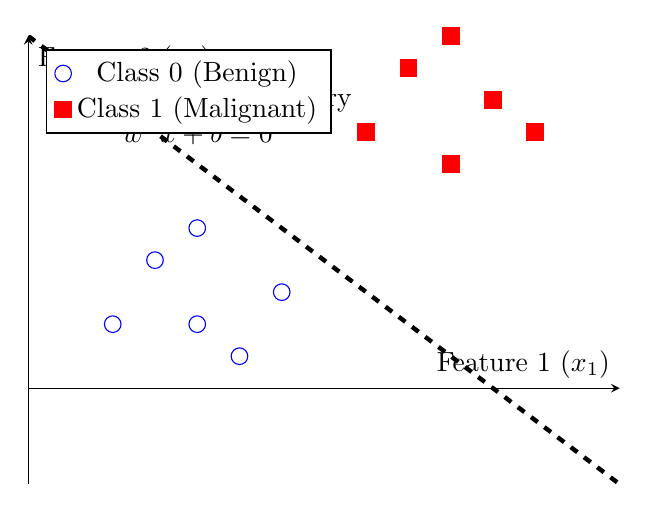
\begin{tikzpicture}
    \begin{axis}[
        xlabel={Feature 1 ($x_1$)},
        ylabel={Feature 2 ($x_2$)},
        axis lines=middle,
        width=0.75\textwidth,
        height=0.6\textwidth,
        xtick=\empty, ytick=\empty,
        legend pos=north west
    ]
    % Class 0 (Blue Circles)
    \addplot[only marks, mark=o, color=blue, mark size=3pt] coordinates {
        (1, 1) (1.5, 2) (2, 1) (2, 2.5) (3, 1.5) (2.5, 0.5)
    };
    \addlegendentry{Class 0 (Benign)}
    
    % Class 1 (Red Squares)
    \addplot[only marks, mark=square*, color=red, mark size=3pt] coordinates {
        (4, 4) (4.5, 5) (5, 3.5) (5.5, 4.5) (6, 4) (5, 5.5)
    };
    \addlegendentry{Class 1 (Malignant)}
    
    % Decision Boundary
    \addplot[domain=0:7, color=black, ultra thick, dashed] {-x + 5.5};
    \node[right] at (axis cs:1, 4.5) {Decision Boundary};
    \node[right] at (axis cs:1, 4) {$w^T x + b = 0$};
    \end{axis}
\end{tikzpicture}
\caption{Geometric View: The decision boundary separates the two classes.}
\label{fig:log_reg_geometry}
\end{figure}

The equation of this boundary is our familiar linear equation:
\begin{equation}
    z = w^T x + b = w_1 x_1 + w_2 x_2 + b
\end{equation}
\begin{itemize}
    \item If a point is on one side ($z > 0$), we predict Class 1.
    \item If a point is on the other side ($z < 0$), we predict Class 0.
    \item If $z = 0$, the point lies exactly on the boundary.
\end{itemize}

% ========================================
% SECTION: PERCEPTRON TRICK
% ========================================
\section{The Precursor: The Perceptron Trick}
Before Logistic Regression, there was the \textbf{Perceptron}. It uses a simple ``Push and Pull'' logic to find the decision boundary.

\subsection{The Algorithm}
\begin{enumerate}
    \item Start with a random line (random weights).
    \item Pick a random data point $(x_i, y_i)$.
    \item If it is \textbf{correctly classified}, do nothing.
    \item If it is \textbf{misclassified}:
    \begin{itemize}
        \item \textbf{Positive point in negative region}: Move the line \textit{towards} the point (Add $x_i$ to weights).
        \item \textbf{Negative point in positive region}: Move the line \textit{away} from the point (Subtract $x_i$ from weights).
    \end{itemize}
\end{enumerate}

\textbf{Unified Update Rule}:
\begin{equation}
    W_{\text{new}} = W_{\text{old}} + \eta (y_i - \hat{y}_i) x_i
\end{equation}

\subsection{Why did we move to Logistic Regression?}
The Perceptron has two major flaws:
\begin{enumerate}
    \item \textbf{No Conviction}: It stops as soon as points are separated, even if the line is barely touching the points. It doesn't find the \textit{best} line, just \textit{any} separating line.
    \item \textbf{Binary Output}: It gives a hard Yes/No, not a probability.
\end{enumerate}

\begin{lstlisting}[language=Python, caption=Perceptron Step Function]
import numpy as np

def perceptron_step(X, y, weights, lr=0.1):
    """Updates weights based on one random point."""
    idx = np.random.randint(0, X.shape[0])
    x_i, y_i = X[idx], y[idx]
    
    # Predict (Step Function)
    y_pred = 1 if np.dot(weights, x_i) >= 0 else 0
    
    # Update: W = W + lr * (y - y_pred) * x
    weights = weights + lr * (y_i - y_pred) * x_i
    return weights
\end{lstlisting}

% ========================================
% SECTION 4: THE SIGMOID FUNCTION
% ========================================
\section{The Sigmoid Function}
We need to convert the output $z$ (which ranges from $-\infty$ to $+\infty$) into a probability (range $[0, 1]$).

\begin{definition}
\textbf{Sigmoid Function} (also called Logistic Function):
\begin{equation}
    \sigma(z) = \frac{1}{1 + e^{-z}}
\end{equation}
\end{definition}

\begin{figure}[htbp]
\centering
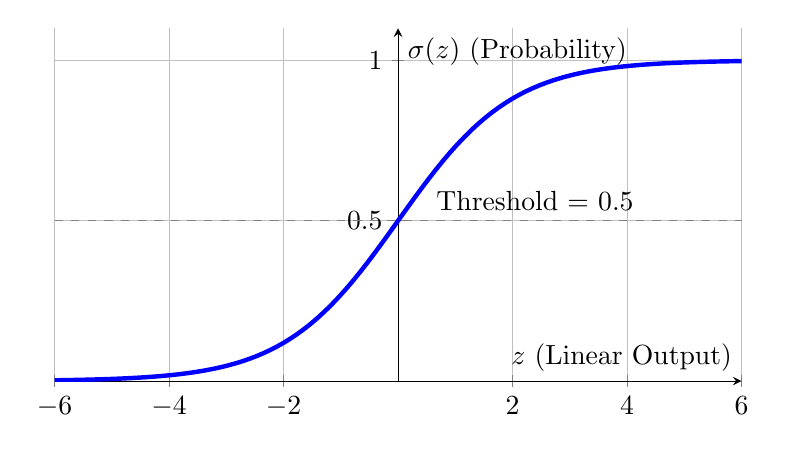
\begin{tikzpicture}
    \begin{axis}[
        xlabel={$z$ (Linear Output)},
        ylabel={$\sigma(z)$ (Probability)},
        xmin=-6, xmax=6,
        ymin=0, ymax=1.1,
        axis lines=middle,
        grid=major,
        width=0.85\textwidth,
        height=0.5\textwidth
    ]
    \addplot[domain=-6:6, color=blue, ultra thick, samples=100] {1/(1+exp(-x))};
    \draw[dashed, gray] (axis cs:-6, 0.5) -- (axis cs:6, 0.5);
    \node[above right] at (axis cs:0.5, 0.5) {Threshold = 0.5};
    \end{axis}
\end{tikzpicture}
\caption{The Sigmoid curve maps any real number to a valid probability between 0 and 1.}
\label{fig:sigmoid}
\end{figure}

\textbf{Key Properties}:
\begin{itemize}
    \item When $z=0$: $\sigma(z) = 0.5$ (Maximum uncertainty).
    \item When $z$ is large positive: $\sigma(z) \approx 1$ (Confident Class 1).
    \item When $z$ is large negative: $\sigma(z) \approx 0$ (Confident Class 0).
    \item The function is smooth and continuously differentiable.
\end{itemize}

% ========================================
% SECTION 5: POLYNOMIAL LOGISTIC REGRESSION
% ========================================
\section{Handling Non-Linear Data: Polynomial Features}
Standard Logistic Regression creates a \textbf{linear} decision boundary. But what if your data is shaped like a circle or a moon?

\textbf{The Trick}: We do NOT change the Logistic Regression algorithm. We change the \textbf{data} by adding polynomial features.

\textbf{Example}: If we have features $x_1$ and $x_2$, we add:
\begin{itemize}
    \item Degree 2: $x_1^2, x_2^2, x_1 \cdot x_2$
    \item Degree 3: $x_1^3, x_2^3, x_1^2 \cdot x_2, x_1 \cdot x_2^2$, etc.
\end{itemize}

The model still sees a linear equation: $z = w_1 x_1 + w_2 x_2 + w_3 x_1^2 + \ldots$

But in the \textit{original} 2D space, this creates a \textbf{curved decision boundary}.

\begin{lstlisting}[language=Python, caption=Polynomial Logistic Regression]
from sklearn.preprocessing import PolynomialFeatures
from sklearn.linear_model import LogisticRegression
from sklearn.pipeline import Pipeline
from sklearn.datasets import make_moons

# Create non-linear data (moon shapes)
X, y = make_moons(n_samples=200, noise=0.1)

# Pipeline: Polynomial Features -> Logistic Regression
model = Pipeline([
    ('poly', PolynomialFeatures(degree=3)),
    ('log_reg', LogisticRegression(max_iter=1000))
])

model.fit(X, y)
print(f"Accuracy: {model.score(X, y):.2f}")  # ~98%
\end{lstlisting}

\textbf{Warning}: High polynomial degrees (e.g., 10+) will \textbf{overfit}. Use cross-validation to find the optimal degree.

% ========================================
% SECTION 6: KEY TAKEAWAYS
% ========================================
\section{Key Takeaways}
\begin{enumerate}
    \item Logistic Regression is a \textbf{classification} algorithm, not regression.
    \item It finds a \textbf{linear decision boundary} to separate classes.
    \item The \textbf{Sigmoid function} converts the linear output to a probability.
    \item The model predicts the \textbf{probability} of belonging to a class, then thresholds at 0.5.
    \item For non-linear data, use \textbf{PolynomialFeatures} to create curved boundaries.
\end{enumerate}

% ========================================
% SECTION 7: HOTS QUESTIONS
% ========================================
\section{HOTS: Interview Questions}
\textbf{Q1: Why is it called ``Logistic Regression'' if it is used for classification?}
\begin{itemize}
    \item Historically, it was derived from regression techniques. The model ``regresses'' the log-odds (logit) of the probability, not the probability itself.
    \item $\text{logit}(p) = \log\left(\frac{p}{1-p}\right) = w^T x + b$
\end{itemize}

\textbf{Q2: Can Logistic Regression handle non-linear decision boundaries?}
\begin{itemize}
    \item By itself, no. It draws a straight line/hyperplane.
    \item However, you can engineer polynomial features (like $x_1^2, x_1 x_2$) to create curved boundaries.
\end{itemize}

\textbf{Q3: What happens if the data is perfectly linearly separable?}
\begin{itemize}
    \item The weights can grow infinitely large, trying to push the sigmoid output to exactly 0 or 1.
    \item Solution: Use \textbf{Regularization} (L2 penalty) to constrain the weights.
\end{itemize}

% ========================================
% SECTION 8: QUICK REFERENCE
% ========================================
\section{Quick Reference Card}

\begin{center}
\fbox{\parbox{0.9\textwidth}{
\textbf{LOGISTIC REGRESSION - CHEAT SHEET}
\vspace{0.3cm}

\textbf{Model}: $P(y=1|x) = \sigma(w^Tx + b) = \frac{1}{1+e^{-(w^Tx+b)}}$

\textbf{Decision Rule}: Predict Class 1 if $P > 0.5$, else Class 0

\textbf{Sigmoid Properties}:
\begin{itemize}
    \item $\sigma(0) = 0.5$ (Max uncertainty)
    \item $\sigma(\pm\infty) \rightarrow 0 \text{ or } 1$ (Confident)
    \item Derivative: $\sigma'(z) = \sigma(z)(1-\sigma(z))$
\end{itemize}

\textbf{Decision Boundary}: $w^Tx + b = 0$ (Linear hyperplane)

\textbf{Non-Linear Data}: Use \texttt{PolynomialFeatures} to curve the boundary

\textbf{Scikit-Learn}: \texttt{LogisticRegression(C=1.0, max\_iter=100)}

\textbf{Interview Gold}:
\begin{itemize}
    \item Name confusion: "Regression" is historical (regresses log-odds)
    \item Separable data $\rightarrow$ weights explode $\rightarrow$ use regularization
    \item Default boundary draws a straight line/hyperplane
\end{itemize}
}}
